\documentclass[11pt,legalpaper]{article}

\usepackage[english]{babel}
\usepackage[utf8]{inputenc}
\usepackage{amsmath}
\usepackage{amssymb}
\usepackage{graphicx}
\usepackage[colorinlistoftodos]{todonotes}
\usepackage{listings,multicol}
\usepackage{textcomp}
\usepackage{hyperref}

\footskip 0cm
\textwidth 17cm
\textheight 32.5cm
\oddsidemargin 0cm
\evensidemargin 0cm
\topmargin -2.5cm


\usepackage[numbered,framed]{matlab-prettifier}
\lstMakeShortInline"
\lstset{
  style              = Matlab-editor,
  %basicstyle         = \mlttfamily,
  escapechar         = ",
  mlshowsectionrules = true,
}



\begin{document}

\title{L1 NUMERICO UDEC}


\begin{minipage}{0.12\textwidth}

\includegraphics[width=\textwidth]{logoudec.eps}
\end{minipage}
\hspace{5mm}
\begin{minipage}{0.9\textwidth}
UNIVERSIDAD DE CONCEPCION\\
{\small\small\bf 
FACULTAD DE CIENCIAS\\ 
FISICAS Y MATEMATICAS}\\
DEPARTAMENTO DE INGENIERIA MATEMATICA\\
\rule{0.80\textwidth}{.5pt} 
\end{minipage}
\vspace*{0.5cm} 

\centerline {\bf\underline{Laboratorio 1, C\'alculo Num\'erico 521230 }}
\centerline{\textrm{Semana 21-29 de marzo de 2018.}}  \vspace{0.2cm}


% \textbf{Nombre:} \hspace{0.5\textwidth}\textbf{Carrera:}
% \vspace{0.1cm}
% \textbf{Profesor:}\hspace{0.5\textwidth} \textbf{ RUT:}
%  \begin{center}
%  \begin{tabular}{||p{2cm}|p{2cm}|p{2cm}||}
%  \hline
%  Pregunta 1 &  Pregunta 2 &     Total\\
%  \hline

%   \vspace{1.5cm} & &       \\
%  \hline
%  \end{tabular}
%  \end{center}
% Enviar documentos solicitados en el formato solicitado a \textbf{veranonumerico@gmail.com}.

\centerline{\textbf{Introducci\'on  a Matlab}\circledR} 
%
\section{Introducci\'on}

MATLAB (abreviatura de \textbf{MAT}rix \textbf{LAB}oratory, "laboratorio de matrices") es una herramienta de 
software matem\'atico que ofrece un entorno de desarrollo integrado (IDE) con un lenguaje de programación propio 
(lenguaje M). Está disponible para las plataformas Unix, Windows, Mac OS X y GNU/Linux .

Entre sus prestaciones básicas se hallan: la manipulación de matrices, la representación de datos y funciones, 
la implementación de algoritmos, la creación de interfaces de usuario (GUI) y la comunicación con programas en 
otros lenguajes y con otros dispositivos hardware. El paquete MATLAB dispone de dos herramientas adicionales 
que expanden sus prestaciones, a saber, Simulink (plataforma de simulación multidominio) y GUIDE 
(editor de interfaces de usuario - GUI). Además, se pueden ampliar las capacidades de MATLAB con las cajas 
de herramientas (toolboxes); y las de Simulink con los paquetes de bloques (blocksets).
%
\section{Ventanas}

La interfaz gr\'afica de MATLAB est\'a organizada en una serie de ventanas, ver figura \ref{fig:interfaz}, 
las cuales pueden ser acopladas dentro de una ventana principal o desacopladas seg\'un el usuario estime conveniente. 
Para acoplarlas o desacoplarlas es suficiente hacer click en un boton de acoplado o desacolpado (``docking'') 
que se representa como una flecha apuntando hacia arriba o hacia abajo y a la derecha, generalmente ubicada en la esquina superior derecha de cada ventana.
\begin{figure}[htp]
\begin{center}
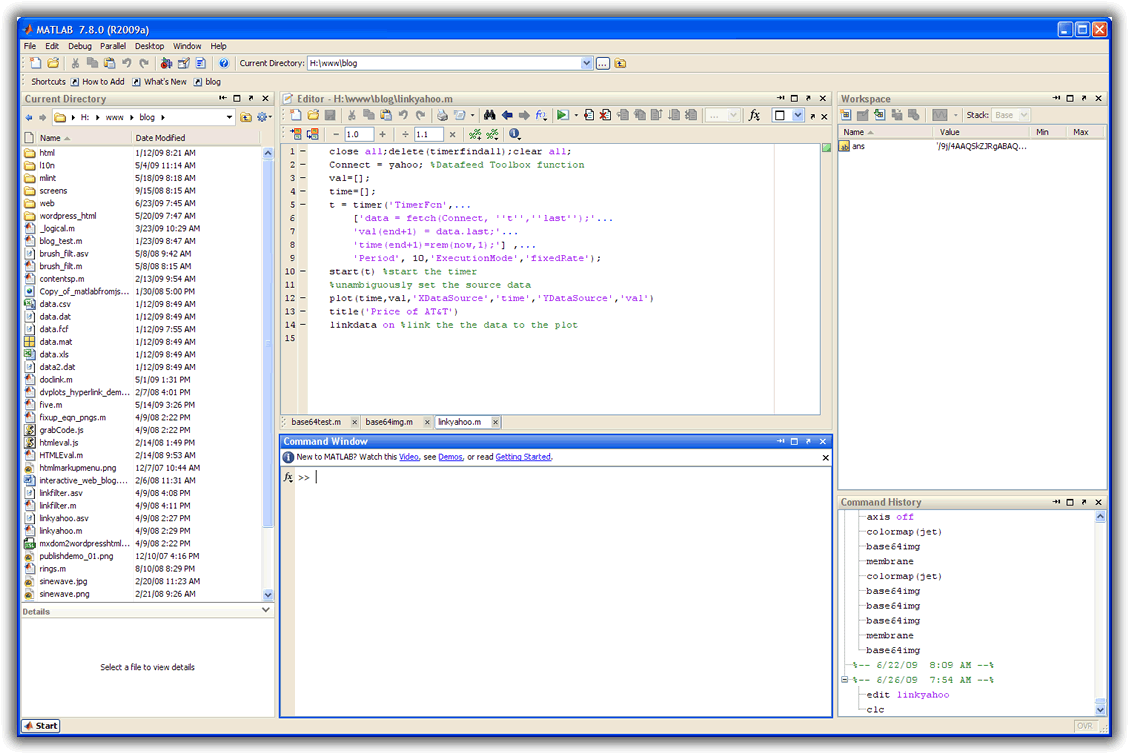
\includegraphics[width=0.8\textwidth]{./M2009desktop.png}
\caption{\sl Interfaz gr\'afica de Matlab y sus ventanas.}
\label{fig:interfaz}
\end{center}
\end{figure}

La \textbf{ventana de comandos} de MATLAB (command window) permite ejecutar instrucciones directamente, en todas la versiones de MATLAB la ventana de comandos muestra los signos 
\begin{verbatim}
 >>
\end{verbatim}
diciendo que lo que el usuario escriba a continuaci\'on ser\'a ejecutado 
inmediatamente. 

La ventana \textbf{lugar de trabajo} (workspace) muestra 
las variables que est\'an actualmente disponibles para ser llamadas. 

La ventana \textbf{directorio actual} (current directory) muestra los archivos 
disponibles en el directorio de trabajo, el directorio de trabajo puede ser cambiado f\'acilmente con la 
barra de navegaci\'on ubicada en la parte superior de la ventana principal.

\subsection{Ventana de comandos}
La ventana de comandos es b\'asicamente una interfaz gr\'afica que permite ejecutar una instrucci\'on de MATLAB.
A modo de ejemplo, empezemos declarando los distintos tipos de variables que usaremos a lo largo de este curso.

La instrucci\'on
\begin{verbatim}
 >> a=1
\end{verbatim}
grabar\'a en memoria local (chequear en la ventana workspace) una variable con el nombre \texttt{a} la cual es un n\'umero 
que tiene el valor 1. Adem\'as, durante la ejecuci\'on MATLAB mostr\'o esta nueva asignaci\'on de la forma.
\begin{verbatim}
>> a=1

a =

     1

>>
\end{verbatim}
Cuando no queramos observar las asignaciones que MATLAB realiza debemos terminar la instrucci\'on con el operador \texttt{;}. 
Por ejemplo, la siguiente instrucci\'on tiene por objeto redefinir la variable anterior y no mostrar esta nueva asignaci\'on.
\begin{verbatim}
>> a=10;
\end{verbatim}
%
\subsection{Ventana del editor}
Otra funcionalidad de MATLAB es su editor. Este editor permite escribir ficheros y funciones en lenguaje M. Para llamar 
al editor se ejecuta directamente en la ventana de comandos, la instrucci\'on es 
\begin{verbatim}
 >> edit
\end{verbatim}
este editor es un editor de texto plano, es decir lo que en \'el se escribe se graba como simples car\'acteres en la memoria. 
El editor permite abrir, grabar, copiar, pegar, editar, escribir, enumerar las l\'ineas y car\'acteres dentro de las l\'ineas y 
adem\'as ejecutar lo escrito directamente en la ventana de comandos. Para hacer uso adecuado del editor, debemos primero conocer 
las funciones y operaciones mas importantes de MATLAB.

El editor tambi\'en puede ser llamado desde la ventana de comandos como
\begin{verbatim}
 >> edit nombre
\end{verbatim}
lo que abre y crea, si es posible, un fichero llamado \textbf{nombre.m} en la carpeta del \textbf{directorio actual}.

\subsection{Ventana del directorio actual}
  En el directorio actual se puede grabar ficheros $.m$ que contengan c\'odigo escrito 
  en lenguaje $M$. Este c\'odigo puede ser ejecutado simplemente llamado desde 
  la ventana de comando el nombre del fichero.
  
  Una de las ventajas de ordenar el trabajo en ficheros es que podemos dividir el c\'odigo en instrucciones que se repiten.
  
Baje el archivo disponible en la siguiente URL y ejec\'utelo. \begin{center}
\url{http://www.udec.cl/~fmilanese/codigo1.m}
\end{center} Para esto, descargue el archivo mencionado y gr\'abelo en la carpeta donde   est\'e ubicado su lugar de trabajo. Luego escriba en la \textbf{ventana de comandos} el  nombre del archivo, puede ser con o sin la extensi\'on. 
  \textquestiondown Qu\'e genera este c\'odigo?. \textquestiondown Le parece conocido?

%
\section{Operaciones l\'ogicas y ciclo while()}
La base de todo lenguaje de programaci\'on son las operaciones l\'ogicas. MATLAB puede realizar todo tipo de operaciones 
l\'ogicas entre variables que sean n\'umeros. Las instrucciones son
\begin{center}
  \begin{tabular}{c|c}
  \hline
  Operador 		& Sentencia \\
  \hline
    o				&  \textbar\textbar \\
    y				& 	\&\&\\	
    o excluyente	& xor()\\
    negaci\'on		& \texttildelow
  \end{tabular}
\end{center}
los valores de verdad en MATLAB se consideran como estados Booleanos, donde se asume que el estado 1 es verdadero 
y el estado 0 es falso. Por ejemplo, las sentencias
\begin{lstlisting}
 1&&1
 1||0
 1||~0
 (~0||1)&&1
 xor(0,~1)
\end{lstlisting}
retornar\'an todas el valor de verdadero. Mientras que las sentencias
\begin{lstlisting}
 1&&0
 ~1||0
 ~1||~~0
 (~0||1)&&0
 xor(1,~1)
\end{lstlisting}
retornar\'an el valor de falso.

Otro principio importante en la matem\'atica es la tricotom\'ia de los n\'umeros reales. Sabemos que dos reales satisfacen siempre 
tres opciones, el primero es mayor que el segundo, el segundo es mayor que el primero o son iguales. Las sentencias 
para verificar la tricotomia de dos variables son
\begin{center}
\begin{tabular}{c|c}
 \hline
 Operador 		& Sentencia \\
 \hline
  igualdad		& $==$\\
  mayor			& $>$\\	
  menor			& $<$\\
  mayor o igual		& $>=$\\
  menor o igual		& $<=$	
\end{tabular}
\end{center}
y se utilizan de la siguiente forma
\begin{lstlisting}
  39==39
  1>0
 -1100<2
 -1<=0
 -1>=-1
\end{lstlisting}
los cuales ser\'an todos valores verdaderos.

Desde los inicios de los computadores interesa que ellos ejecuten instrucciones durante ciertas condiciones. Esto 
se maneja con un ciclo llamado ``while'' (del ingl\'es durante). Haremos uso de lo hasta ahora visto para entender el 
siguiente c\'odigo.
\begin{lstlisting}
a=0;
b=1;
while(a<10)
  b=b+1;
  a=a+2;
end
\end{lstlisting}
Al final de esta instrucci\'on se observa que al variable $a$ tiene el valor 10 mientras que $b$ tiene el valor 6.
(\textquestiondown Por qu\'e?). Un error sumamente com\'un aparece cuando aparece en el uso de estos ciclos while, si la 
condici\'on expresada entre par\'entesis siempre es verdadera el ciclo while no terminar\'a, lo que deja al computador 
realizando un trabajo que nunca termina, por ejemplo, si modificamos el c\'odigo anterior seg\'un 
\begin{lstlisting}
a=0;
b=1;
while(a<10)
  b=b+1;
  a=a-2;
end
\end{lstlisting}
la instrucci\'on no terminar\'a nunca y MATLAB aparentar\'a que est\'a detenido, pero en realidad est\'a trabajando al m\'aximo 
en la tarea infinita que le asignamos. Para detener este procedimiento basta presionar los botones \texttt{cntrl+c}, esta 
instruccion deteniende cualquier ejecuci\'on de MATLAB en cualquier momento. Es importante observar que si dejamos 
ejecutar el c\'odigo anterior, durante un tiempo prolongado, las variables \texttt{a} y \texttt{b} empezar\'an a tomar valores 
cada vez mas grandes y que para ser almacenados en memoria requieren cada vez mas espacio y eventualmente se agotar\'a la memoria 
RAM disponible en el ordenador, en este caso MATLAB dir\'a:
\begin{verbatim}
Out of memory. Type HELP MEMORY for your options.
\end{verbatim}
%
\section{Condicion if()}
Otra instrucci\'on importante es la de los ciclos condicionales. Es decir, cuando se sujeta cierta 
ejecuci\'on del c\'odigo a que se satisfaga cierta condici\'on. En matlab la estructura es sumamente sencilla 
y queda expresada f\'acilamente en el siguiente c\'odigo.
\begin{lstlisting}
 a=1;
  if a==0
    b=0;
  else
    b=33;
  end
\end{lstlisting}
el cual crear\'a la variable $b$ con el valor $33$ puesto que $a$ no es cero. Tambi\'en se puede usar una versi\'on multicondicional 
la cual se opera seg\'un:
\begin{lstlisting}
 a=22;
  if a==0
    b=33;
  elseif a>10
    b=7;
  elseif a==22
    b=33;
  else
    b=0
  end
\end{lstlisting}
la cual crear\'a la variable b=7, puesto que en primer lugar a no es cero y luego a si es mayor que 10. Notar que el ciclo 
de condicional no asignar\'a a b e valor 33, puesto que se satisface primero el segundo condicional ``$a>10$''.
%
\section{Vectores y matrices}
No debemos olvidar que MATLAB son las siglas de laboratorio de matrices. Existen varias formas de declarar un vector o matriz, 
para empezar debemos considerar que cuando hacemos una asignaci\'on de un n\'umero a una variable, lo que estamos haciendo es 
construir una matriz de orden 1. Es decir, todo lo anterior fue realizado con matrices. Supongamos que queremos 
ingresar la matriz
$$
\left [
  \begin{array}{cc}
    33 & 44 \\
    1  & 0
  \end{array}
\right ],
$$
en tal caso debemos ejecutar la siguiente sentencia
\begin{verbatim}
 A=[33,44;1,0];
\end{verbatim}
tambi\'en podemos ingresar matrices construyendolas a partir de sus \'indices, as\'i podriamos ingresar 
\begin{lstlisting}
 B(1,1)=33;
 B(1,2)=44;
 B(2,1)=1;
 B(2,2)=5;
\end{lstlisting}
y si realizamos la instrucci\'on de comparaci\'on de estas dos matrices obtendremos
\begin{verbatim}
 >> A==B

ans =

     1     1
     1     1
     
\end{verbatim}
esta salida es una matriz del mismo orden que $A$ y $B$ pero la cual tiene puros valores verdadero 
en todas sus componentes. Puesto, efectivamente $A$ es igual a $B$ en todas sus componentes.

Se pueden generar tambi\'en vectores y matrices de forma mas compacta usando el operador $:$, por ejemplo 
la instrucci\'on 
\begin{verbatim}
 a=1:100;
\end{verbatim}
crear\'a en memoria un vector de largo 100, que empieza en el 1 y termina en el 100. Si queremos que el avance sea de 
dos en dos, podemos ejecutar
\begin{verbatim}
 a=1:2:100;
\end{verbatim}
y ahora el vector $a$ es un vector de largo 50, que empieza en el 1 y termina en el 99. Otra forma de declarar un vector 
es usando la instrucci\'on \texttt{linspace()}. Por ejemplo, podriamos haber definido este \'ultimo vector usando 
linspace seg\'un
\begin{verbatim}
 a=linspace(1,99,50);
\end{verbatim}

Algunas operaciones que se pueden realizar con matrices son.

\begin{center}
\begin{tabular}{l|l}
\hline
Comando		& Significado \\
\hline
\texttt{inv(M)}	&  	Inversa de la matriz M		\\
\texttt{M'}		& 	Transpuesta de la matriz M	\\
\texttt{det(M)}	&	Determinante de la matriz M	\\
\texttt{M(2,3)}	&	El elemento en la posici\'on (2,3) de la matriz M\\
\texttt{M(:,2)}	&	Segunda fila de M\\
\texttt{M(3,:)}	&	Tercera columna de M\\
\texttt{M(1:2,1)}&	Los elementos desde el 1 al 2 de la primera columna de M\\
\texttt{[m,n]=size(M)}& Dimensi\'on de M, n\'umero de filas m y columnas n
\end{tabular}
\end{center}

\subsection{Funciones para la construcci\'on de matrices}

A continuaci\'on, algunos comandos que permiten construir matrices preestablecidas.

\begin{center}
\begin{tabular}{l|p{0.8\textwidth}}
\hline
Comando		& Significado \\
\hline
\texttt{eye(3)}		& Matriz identidad de orden 3\\
\hline
\texttt{ones(4)} 	& Matriz de orden 4 de puros unos\\
\hline
\texttt{zeros(3)} 	& Matriz de ceros de orden 3\\
\hline
\texttt{diag(M)} 	& Crea una matriz diagonal a partir de un vector M,
la cual contiene los elementos de M en su diagonal.\\
& Si la entrada M es una matriz, entonces este comando entrega un vector cuyos elementos son la\\
& diagonal de la matriz M\\
\hline
\texttt{triu(M)}& Parte triangular superior  de una matriz M \\
\hline
\texttt{tril(M)}& Parte triangular inferior de una matriz M\\
\hline
\texttt{rand(n,m)}& Matriz aleatoria con valores entre 0 y 1 de orden $n\times m$
\end{tabular}
\end{center}


\subsection{Concadenaci\'on de matrices y vectores}
Otra caracter\'istica peculiar de MATLAB es la capacidad de concadenar vectores y matrices. Por ejemplo, 
podemos concadenar dos vectores para construir una matriz seg\'un
\begin{verbatim}
 a=[1;2]
 b=[3;4]
 A=[a,b]
\end{verbatim}
esto se puede interpretar como juntar los vectores $a$ y $b$ en una nueva matriz, dejando  $b$ a la derecha de $a$ 
y llamando a esta matriz $A$. Si intentamos realizar una concadenaci\'on que no tiene sentido, como por ejemplo
\begin{verbatim}
 a=[3,2]
 b=[3;4]
 A=[a;b]
\end{verbatim}
MATLAB nos dir\'a 
\begin{verbatim}
Error using vertcat
Dimensions of matrices being concatenated are not consistent.
\end{verbatim}
por que efectivamente, la instrucci\'on que le ordenamos a MATLAB fue adjunta a la derecha del vector fila $a$ 
el vector columna $b$, lo cual deja una secci\'on de informaci\'on indefinida.

Los comandos vistos anteriormente para la construcci\'on de ciertas matrices se pueden combinar para formar matrices m\'as complejas de forma m\'as simple. Por ejemplo, las instrucciones

\begin{center}
\begin{tabular}{l|p{0.6\textwidth}}
\texttt{A=[1 2 3 ;3 4 5];}
	& Concadenaci\'on de dos vectores y creaci\'on de matriz A\\
\texttt{B=[-1 -2 -3;A;ones(1,3)];}
	&Concadenaci\'on de una matriz y dos vectores\\
\texttt{C=[eye(4) zeros(4,3);zeros(4,4) B];} 
	& Esto se llama ensamblamiento por bloques\\
\texttt{D=diag(diag(C));}
	& Extracci\'on de un vector diagonal\\
\end{tabular}
\end{center}

%
\subsection{Indexaci\'on y llenado de una matriz}
Recordemos que una matriz est\'a indexada y que estos \'indices puede ayduarnos a definir los valores de una matriz. 
Una caracter\'istica de MATLAB es que podemos extraer ciertos \'indices e inclusive recorrerlos en un orden predefinido, 
por ejemplo las siguientes sentencias
\begin{lstlisting}
 v=[1:4,33,44,-1:2];
 vI=v(1:2:end)
 vI2=v(1:3:end-1)
 vR=v(end:-1:1)
\end{lstlisting}
retornar\'an
\begin{verbatim}
vI =

     1     3    33    -1     1


vI2 =

     1     4    -1


vR =

     2     1     0    -1    44    33     4     3     2     1
\end{verbatim}
las cuales son respectivamente la extracci\'on de dos en dos desde el principio hasta el final del vector
\texttt{v}, la extracci\'on de tres en tres, desde el principio hasta el pen\'ultimo del vector \texttt{v},
y la reescritura desde el final hasta el principio del vector \texttt{v}.




\section{Ciclo for()}

Otro ciclo como \texttt{while()}, que resulta de mucho inter\'es, es el ciclo \texttt{for()}. Este ciclo tiene por prop\'osito recorrer un arreglo y ejecutar una setencia a lo largo de este arreglo, por ejemplo, la instrucci\'on:
\begin{lstlisting}
 a=1:4;
 for(i=a)
    2*i
 end
\end{lstlisting}
retornar\'a
\begin{verbatim}
ans =

     2


ans =

     4


ans =

     6


ans =

     8

\end{verbatim}
es decir, los dobles de las componentes del vector $a$. Tambi\'en es posible recorrer las entradas de una matriz, \textquestiondown En que orden recorre el ciclo \texttt{for()} de Matlab las entradas de una matriz?.

\section{Cadenas}
Matlab posee integradas operaciones y funciones que permite trabajar letras, signos y caracteres distintos de números. La agrupación de estos signos forma el tipo de dato \texttt{cadena} ó \texttt{string}. Por ejemplo, la instrucci\'on
\begin{verbatim}
S = 'Cualquier caracter'
\end{verbatim}
crea un arreglo de caracteres. El arreglo es realmente un vector que contiene la codificación numérica en formato Unicode o ASCII, donde el largo de \texttt{S} es el número de caracteres en el arreglo. El caractér de comillas se representa con el de doble apostrofe, por ejemplo
\begin{verbatim}
S = 'Quijote: "¿Donde estás Dulcinea?"'
\end{verbatim}
Todas las operaciones vistas para vectores se pueden realizar para arreglos de caractéres. A modo de ejemplo,
\begin{lstlisting}
nombre='Rodrigo';
apellido='Riquelme';
destinatario=['Sr',nombre,apellido];
alreves=destinatario(end:-1:1);
[destinatario;alreves]
\end{lstlisting}
retornan al ser interpretadas
\begin{verbatim}
>> 

ans =

SrRodrigoRiquelme
emleuqiRogirdoRrS
\end{verbatim}
Hay que tener mucho cuidado cuando en un código trabajamos con números y letras, si bien el número y letra \texttt{0} podemos leerlo igual, en memoria se representa de forma distinta y con ellos se realizan operaciones muy diferentes. Por ejemplo, las siguientes sentencias contienen errores conceptuales
\begin{multicols}{2}
\begin{lstlisting}
>> a=[0,1;2,3];
b='a';
a+b

ans =
    97    98
    99   100
\end{lstlisting}

\begin{lstlisting}
>> b=[0,'1',2];
b==[0,1,2]

ans =

     1     0     1
     
\end{lstlisting}
\end{multicols}
Algunas funciones para trabajar con cadenas 
\begin{center}
\begin{tabular}{l|p{0.8\textwidth}}
\hline
Comando		& Significado \\
\hline
[$s_1,s_2$] \'o \texttt{strcat}($s_1,s_2$)	& Concadena por filas a las cadenas $s_1,s_2$.\\
\hline
\texttt{num2str(x)}	& Convierte a cadena el número almacenado en la variable $x$\\
\hline
\texttt{char(x)} 	& Retorna el caracter que corresponde al número $x$ en código ASCII\\
\hline
\texttt{double(s)} 	& Retorna los número que representan a la cadena $s$ en c\'odigo ASCII\\
\hline 
\end{tabular}
\end{center}

\section{Celdas}
Otro tipo de variable, en el cual es posible combinar, reunir y anidar todos los tipos de variables vistos anteriormente es el tipo celda ó \texttt{cell}. La declaraci\'on de una celda se hace con los caracteres reservados \texttt{\{ \}}. Por ejemplo, la instrucci\'on
\begin{verbatim}
>> a={}

a = 

     {}
\end{verbatim}
crea, almacena y muestra una variable que contiene a una celda vacía o sin contenido. Mientras que la instrucci\'on
\begin{verbatim}
>> a={'1',[1,2;3,4],'cadenas'}

a = 

    '1'    [2x2 double]    'cadenas'
\end{verbatim}
crea, almacena y muestra una variable que contiene una matriz de orden dos y dos cadenas. Para poder acceder a estos elementos, podemos hacer las siguientes instrucciones 
\begin{verbatim}
>> a(1,1),a(1,2),a(1,3)

ans = 

    '1'


ans = 

    [2x2 double]


ans = 

    'cadenas'
\end{verbatim}
donde se extraen los componentes de la celda \texttt{a} como subceldas de este. Mientras que su queremos acceder al contenido que hay en cada una de las celdas de \texttt{a} debemos ejecutar
\begin{verbatim}
>> a{1,1},a{1,2},a{1,3}

ans =

1


ans =

     1     2
     3     4


ans =

cadenas
\end{verbatim}
Lo más interesante de las celdas, es que a diferencia de todos los otros tipos de variables de Matlab, se pueden crear celdas que contengan celdas. Por ejemplo las instrucciones 
\begin{verbatim}
>> a={'1'};
b={a,a};
c={a,b,a}

c = 

    {1x1 cell}    {1x2 cell}    {1x1 cell}
\end{verbatim}
construyen una celda de celdas \texttt{c}. \textquestiondown Cu\'al es el valor de \texttt{c(1,2)} y \texttt{c\{1,2\}}?.

%\newpage
\section{Ejercicios}
  \begin{enumerate}
  	\item Haga un algoritmo que construya, en una matriz, la tabla de multiplicar de 124 filas y 348 columnas.
    \item Construya, usando un ciclo \texttt{for()}, una matriz triangular superior de puros $1$.
   \item Escriba un c\'odigo que construya una matriz de orden $98\times 10$ cuyas filas sean los n\'umero del 1 al 10 y viceversa, alternadamente, es 
   decir
	$$
	\left [
	     \begin{array}{ccc}
	      1 & 2 & 3 \cdots  \\
	      10 & 9 & 8 \cdots \\
     	      1 & 2 & 3 \cdots  \\
	      10 & 9 & 8 \cdots \\
	      \vdots & \vdots & \vdots
	     \end{array}
	\right]
	$$
  \item Escriba un c\'odigo que gire una matriz 90 grados en sentido antihorario.
  
  \item Describa las caracter\'siticas de la variable $A$ en cada uno de los siguientes c\'odigos.
	\begin{multicols}{2}
    \begin{itemize}
     \item[a)] 
\begin{verbatim}
for i=1:10
  for j=1:10
    A(i,j)=1;
  end
end
\end{verbatim}
      \item[b)] 
\begin{verbatim}
for i=1:10
  for j=1:10
      if(i>j)
      A(i,j)=1;
      else
      A(i,j)=-1;
      end
  end
end
\end{verbatim}
      \item[c)] 
\begin{verbatim}
for i=1:10
  for j=1:10
      if(i>2*j)
      A(i,j)=1;
      else
      A(i,j)=-1;
      end
  end
end
\end{verbatim}

   \item[d)] 
\begin{verbatim}
for i=1:10
  j=1;
  while j<7
      if(i>2*j)
      A(i,j)=1;
      else
      A(i,j)=-1;
      end
      j=j+1;
  end
end
\end{verbatim}

   \item[e)] 
\begin{verbatim}

A(1:10,1)=3;
for i=1:10
  j=1;
  while j<2
      if(i>1&&i<3)
      A(i,j)=A(i,j)+1;
      else
      A(i,j)=0;
      end
      j=j+1;
  end
end
\end{verbatim}

   \item[d)] 
\begin{verbatim}
A=1;
for i=1:10
  A(:,end+2)=1
  A(end+1,:)=0;
end
\end{verbatim}
    \end{itemize}
	\end{multicols}
    
    \item Identifique errores l\'ogicos en los siguientes c\'odigos e interprete alg\'un posible significado.
    
    \begin{multicols}{2} 
      \begin{itemize}
       \item[a)]
\begin{verbatim}
 j=0;
 while j>=0
  A(j)=A(j)+1;
 end
\end{verbatim}

       \item[b)]
\begin{verbatim}
A=[1,2;3,4];
B=[A;1,2];
C=[[1;2],A];
D=[[A]];
\end{verbatim}

       \item[c)]
\begin{verbatim}
for i=0:3
  for j=0:3
  A(i,j)=i*j;
  end
end
\end{verbatim}

       \item[d)]
\begin{verbatim}
j=-9;
while j>10
    A(j)=10;
end
\end{verbatim}

       \item[e)]
\begin{verbatim}
i=0;
count=i;
while count<=i
    A(i)=8;
    i=i+1;
    count=i-1;
end
\end{verbatim}
\end{itemize}
    \end{multicols}
\item Cree un c\'odigo que permita intercalar a los caracteres de una cadena la sucesi\'on de caracteres \texttt{+ * / \$}.
\item Construya un rutero que escriba todas las posibles combinaciones de nombres completos de personas que tengan por primer o segundo nombre $\{Juan,\, Diego, Roberto, Antonio\}$ y por apellidos $\{Rodriguez,\, Matamala,\, Riquelme\}$.
      
  \end{enumerate}
  
\end{document}  